\documentclass[14pt,a4paper,report]{report}
\usepackage[a4paper, mag=1000, left=2.5cm, right=1cm, top=2cm, bottom=2cm, headsep=0.7cm, footskip=1cm]{geometry}
\usepackage[utf8]{inputenc}
\usepackage[english,russian]{babel}
\usepackage{indentfirst}
\usepackage[dvipsnames]{xcolor}
\usepackage[colorlinks]{hyperref}
\usepackage{listings} 
\usepackage{fancyhdr}
\usepackage{caption}
\usepackage{amsmath}
\usepackage{graphicx}
\usepackage{amsmath}
\usepackage{booktabs}
\usepackage{array}
\newcolumntype{P}[1]{>{\centering\arraybackslash}p{#1}}
\hypersetup{
	colorlinks = true,
	linkcolor  = black
}

\usepackage{titlesec}
\titleformat{\chapter}
{\Large\bfseries} % format
{}                % label
{0pt}             % sep
{\huge}           % before-code


\DeclareCaptionFont{white}{\color{white}} 

% Listing description
\usepackage{listings} 
\DeclareCaptionFormat{listing}{\colorbox{gray}{\parbox{\textwidth}{#1#2#3}}}
\captionsetup[lstlisting]{format=listing,labelfont=white,textfont=white}
\lstset{ 
	% Listing settings
	inputencoding = utf8,			
	extendedchars = \true, 
	keepspaces = true, 			  	 % Поддержка кириллицы и пробелов в комментариях
	language = C,            	 	 % Язык программирования (для подсветки)
	basicstyle = \small\sffamily, 	 % Размер и начертание шрифта для подсветки кода
	numbers = left,               	 % Где поставить нумерацию строк (слева\справа)
	numberstyle = \tiny,          	 % Размер шрифта для номеров строк
	stepnumber = 1,               	 % Размер шага между двумя номерами строк
	numbersep = 5pt,              	 % Как далеко отстоят номера строк от подсвечиваемого кода
	backgroundcolor = \color{white}, % Цвет фона подсветки - используем \usepackage{color}
	showspaces = false,           	 % Показывать или нет пробелы специальными отступами
	showstringspaces = false,    	 % Показывать или нет пробелы в строках
	showtabs = false,           	 % Показывать или нет табуляцию в строках
	frame = single,              	 % Рисовать рамку вокруг кода
	tabsize = 2,                  	 % Размер табуляции по умолчанию равен 2 пробелам
	captionpos = t,             	 % Позиция заголовка вверху [t] или внизу [b] 
	breaklines = true,           	 % Автоматически переносить строки (да\нет)
	breakatwhitespace = false,   	 % Переносить строки только если есть пробел
	escapeinside = {\%*}{*)}      	 % Если нужно добавить комментарии в коде
}

\begin{document}

\def\contentsname{Содержание}

% Titlepage
\begin{titlepage}
	\begin{center}
		\textsc{Санкт-Петербургский Политехнический 
			Университет Петра Великого\\[5mm]
			Кафедра компьютерных систем и программных технологий}
		
		\vfill
		
		\textbf{Отчёт по лабораторной работе №3.1\\[3mm]
			Курс: «Разработка экспертной системы на базе представленного описания»\\[41mm]
		}
	\end{center}
	
	\hfill
	\begin{minipage}{.4\textwidth}
		Выполнил студент:\\[2mm] 
		Ерниязов Т.Е.\\
		Группа: 13541/2\\[5mm]
		
		Проверил:\\[2mm] 
		Болсуновская М.В.
	\end{minipage}
	\vfill
	\begin{center}
		Санкт-Петербург\\ \the\year\ г.
	\end{center}
\end{titlepage}

% Contents
\tableofcontents
\clearpage

\chapter{Лабораторная работа №3.1}

\section{Цель работы}

Научиться создавать экспертные системы с помощью конструктора Exsys CORVID.

\section{Программа работы}

\begin{itemize}
	\item На примере ОДНОЙ ИЗ ЭС экспертной системы (примеры ЭС выбрать самостоятельно исходя из демо примеров с сайта ExSys Corvid) укажите содержание следующих компонентов:  диалогового компонента, решателя, базы данных, базы знаний).
	\item Выполните лабораторные работы 1-6 из методических рекомендаций Д.И. Муромцев.
	Оболочка экспертных систем Exsys Corvid. – СПб: СПб ГУ ИТМО, 2006. – 69 с. В случае необходимости используйте методические рекомендации от разработчика.
	\item Разработайте статическую экспертную систему для нахождения характерных неисправностей прибора Диск-250 ДД и метода их решения. Прибор показывающий и регистрирующий Диск-250 ДД предназначен для измерения и регистрации силы тока, а также неэлектрических величин, преобразованных в силу тока. Данная ЭС предназначена для использования слесарями в целях быстрого обнаружения неисправности и ее устранения.
\end{itemize}

\clearpage

\section{Ход работы}

\subsection{На примере одной из ЭС с сайта ExSys Corvid укажите содержание следующих компонентов:  диалогового компонента, решателя, базы данных, базы знаний}

Экспертная система: Restaurant Advisor Expert System

\begin{table}[h!]
	\begin{tabular}{ | P{6cm} | P{10cm} | }
		\hline
		Диалоговый компонент & Java-Applet \\ \hline
		База данных & Конкретные рестораны хранящиеся в базе данных. \\ \hline
		База знаний & Набор статических инструкций. \\ \hline
		Решатель & Формирователь правил, которые приводят к подбору подходящего ресторана. Данные для решения берутся из БД и БЗ. \\ \hline
	\end{tabular}
	\caption{Компоненты системы Restaurant Advisor Expert System}
	\label{table:1}
\end{table}

\subsection{Выполнение лабораторных работ 1-6 из методических рекомендаций Д.И. Муромцевй}

\subsubsection{Лабораторная работа №1. Создание простейшей системы}

Разработаем простейшую экспертную систему, работающую по следующему алгоритму:

\begin{lstlisting}
IF
    Свет в Вашем доме внезапно перестал работать
THEN
    замените лампочку

IF
    Свет в Вашем доме продолжает работать
THEN
    Ничего не делать
\end{lstlisting}

Результат конструирования экспертной системы по методическим указаниям:

\begin{figure*}[ht!]
	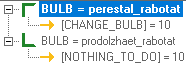
\includegraphics[width=.35\textwidth]{images/1_1.png}\hfill
	
\includegraphics[width=.55\textwidth]{images/1_2.png}
	\caption{Логический и командный блоки}
\end{figure*}

\begin{figure*}[ht!]
	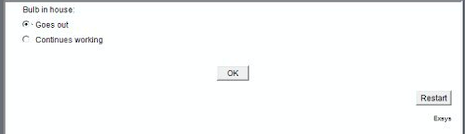
\includegraphics[width=.50\textwidth]{images/1_3.png}\hfill
	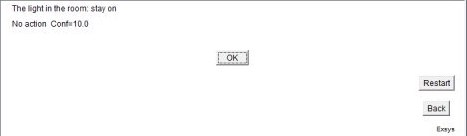
\includegraphics[width=.50\textwidth]{images/1_5.jpg}
	\caption{Если свет продолжает работать, то ничего не делать}
\end{figure*}



\subsubsection{Лабораторная работа №2. Улучшение интерфейса пользователя}

Результат работы улучшения интерфейса пользователя экспертной системы по методическим указаниям:

\begin{figure}[h!]
	\centering
	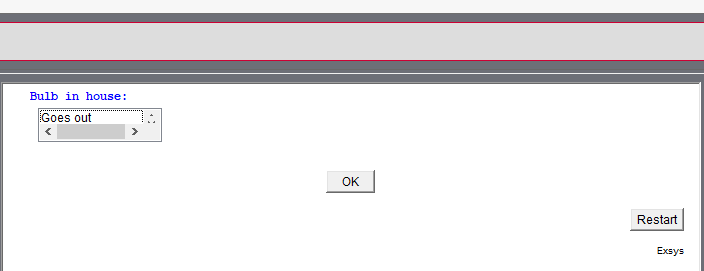
\includegraphics[scale = 0.75]{images/2_1.png}
	\caption{Изменение текста и шрифта выводимого текста}
\end{figure}

\begin{figure}[h!]
	\centering
	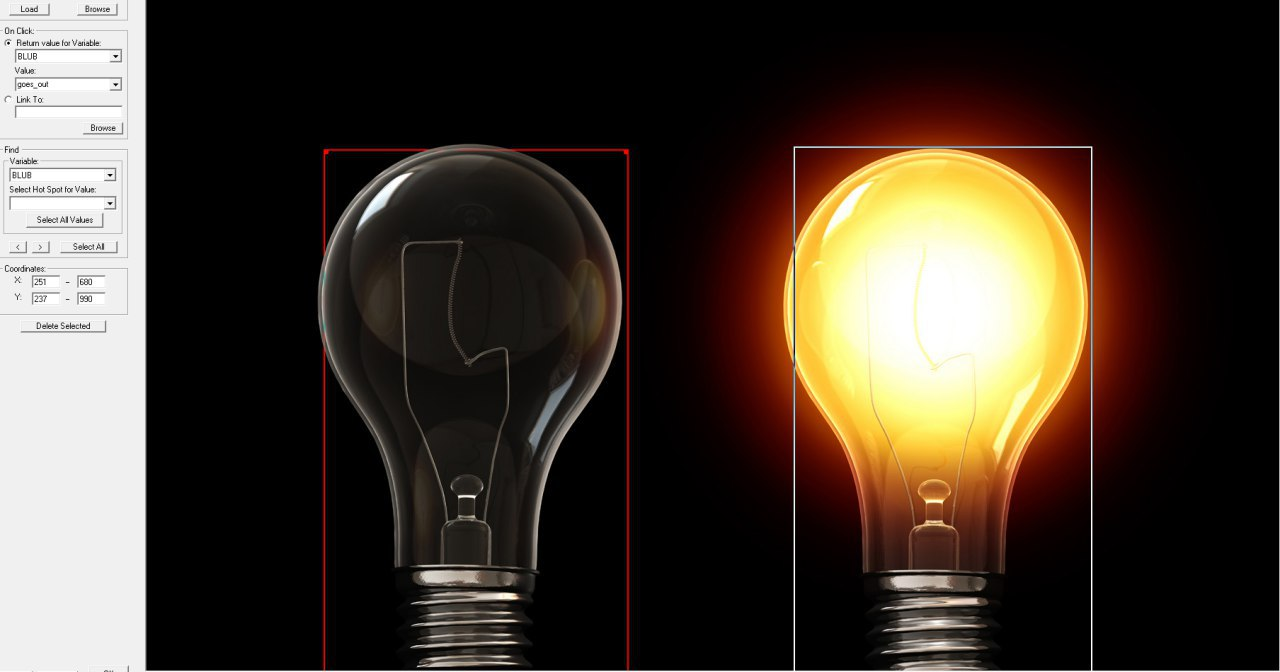
\includegraphics[scale = 0.50]{images/2_2.png}
	\caption{Определение областей для графической карты}
\end{figure}

К сожалению, программа не позволяет запустить проект после установки областей на графической карте, что объясняется либо неточностью методических указаний или багом в программе.

\subsubsection{Лабораторная работа №3. Усиление логики работы системы}

Расширим логику созданной экспертной системы:

\begin{figure}[h!]
	\centering
	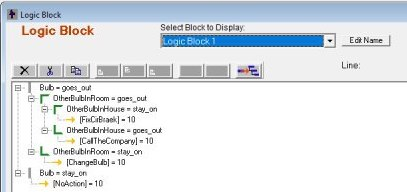
\includegraphics[scale = 0.85]{images/3_1.jpg}
	\caption{Результирующий логический блок}
\end{figure}



\begin{figure*}[h!]

	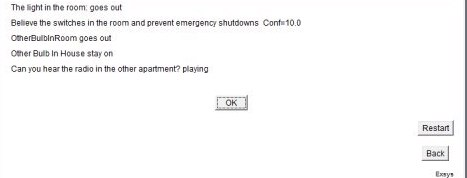
\includegraphics[width=1\textwidth]{images/3_7.jpg}
	\caption{Если другие лампочки в доме продолжают гореть, то надо проверить выключатели}
\end{figure*}

\begin{figure}[h!]
	\centering
	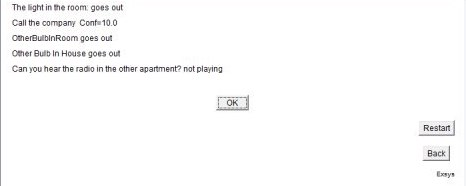
\includegraphics[scale = 1]{images/3_8.jpg}
	\caption{Если другие лампочки в доме погасли, то надо позвонить поставщику электроэнергии}
\end{figure}

\subsubsection{Лабораторная работа №4. Обратная связь}

Реализуем дополнительный логический блок обратной связи:

\begin{figure}[h!]
	\centering
	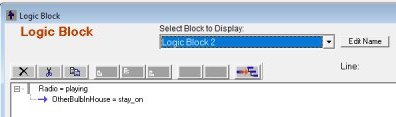
\includegraphics[scale = 0.9]{images/4_1.jpg}
	\caption{Логический блок для реализации обратной связи}
\end{figure}

Система автоматически вызывает окно, спрашивающее пользователя о радио за стеной. Если радио работает, то с электричеством в доме все в порядке.


\begin{figure}[h!]
	\centering
	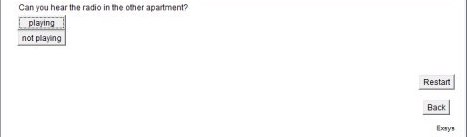
\includegraphics[scale = 0.9]{images/4_2.jpg}
	\caption{Если слышно радио в другой комнате, то другие лампочки в доме продолжают гореть}
\end{figure}


\subsubsection{Лабораторная работа №5. Числовые переменные и [[]] подстановки}

Используем числовую переменную, которая отвечает за мощность лампочки:

\begin{figure}[h!]
	\centering
	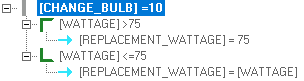
\includegraphics[scale = 1.1]{images/5_1.png}
	\caption{Дополнение логического блока переменной}
\end{figure}

Если мощность больше 75 ватт, то предлагается использовать лампочку 75 ватт. Если меньше, то столько сколько указал пользователь.

\begin{figure*}[ht!]
	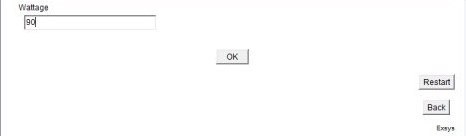
\includegraphics[width=.55\textwidth]{images/5_2.jpg}\hfill
	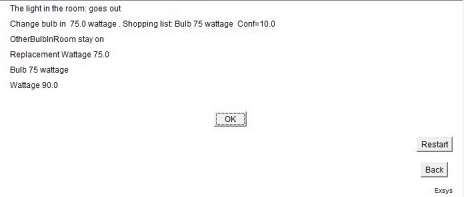
\includegraphics[width=.45\textwidth]{images/5_3.jpg}
	\caption{Если мощность больше 75 ватт, то предлагается использовать лампочку 75 ватт}
\end{figure*}


\begin{figure*}[h!]
	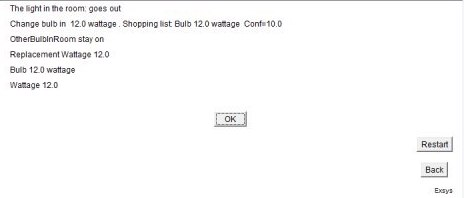
\includegraphics[width=.80\textwidth]{images/5_5.jpg}
	\caption{Если меньше 75 ватт, то столько сколько указал пользователь}
\end{figure*}

Результат свидетельствует о том, что в коллекцию успешно добавилась необходимая запись.


\subsubsection{Лабораторная работа №6. Переменные коллекции}

Используем коллекцию для добавления записи в список покупок. 

\begin{figure}[h!]
	\centering
	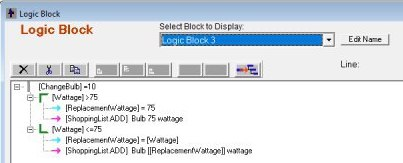
\includegraphics[scale = 1.1]{images/6_1.jpg}
	\caption{Дополнение логического блока коллекцией}
\end{figure}

В результирующем диалоге будет выводиться весь список покупок.


\subsection{Разработка статической экспертной системы для нахождения характерных неисправностей прибора Диск-250 ДД и метода их решения}

Описание разрабатываемой экспертной системы для нахождения характерных неисправностей прибора Диск-250 ДД и метода их решения:

\begin{figure}[h!]
	\centering
	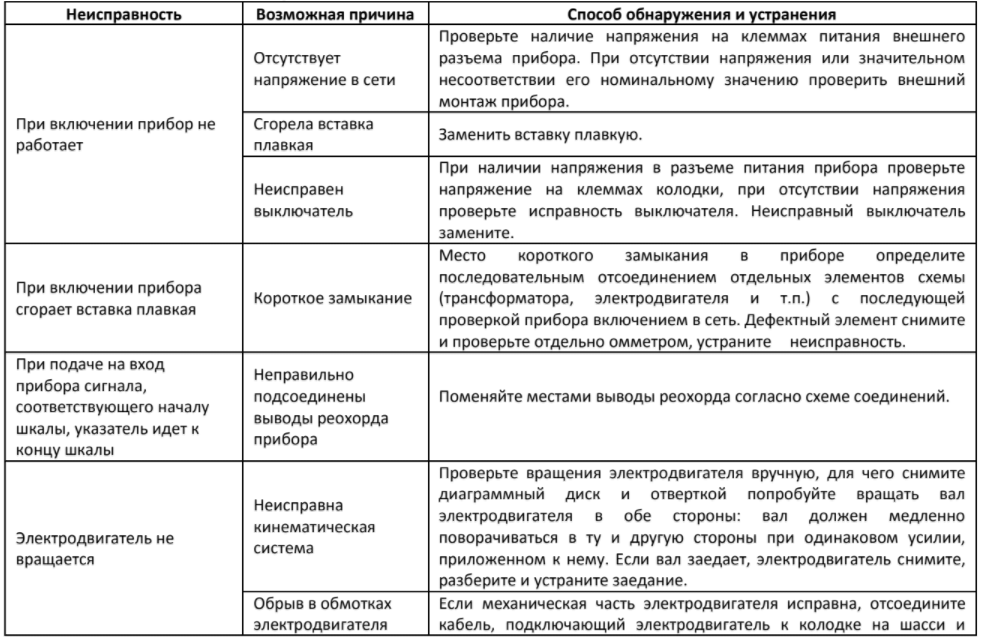
\includegraphics[scale = 0.65]{images/7_x1.png}
\end{figure}

\begin{figure}[h!]
	\centering
	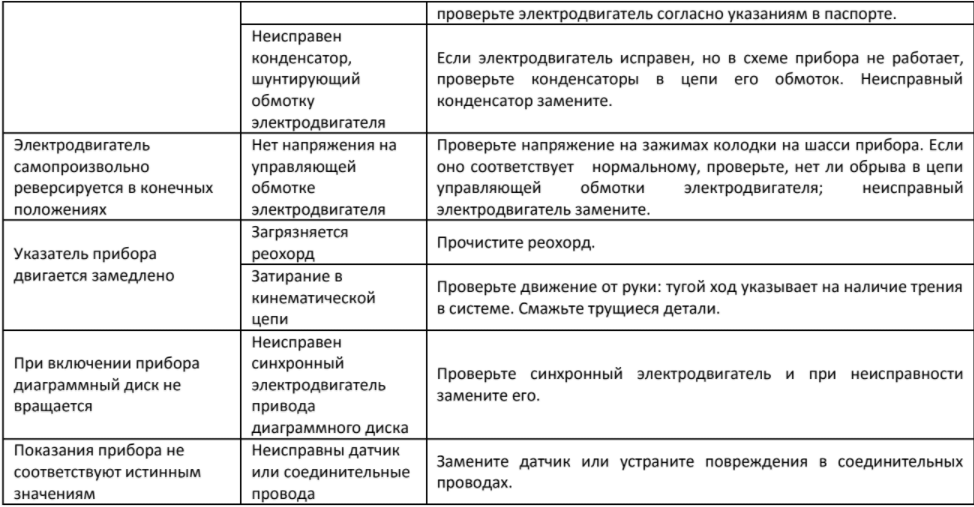
\includegraphics[scale = 0.65]{images/7_x2.png}
\end{figure}

\clearpage
На основе описания экспертной системы создаем переменные и логический блок:

\begin{figure}[h!]
	\centering
	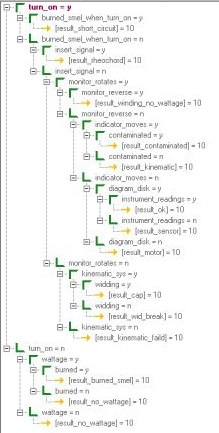
\includegraphics[scale = 1.35]{images/1.jpg}
	\caption{Логический блок заданной экспертной системы}
\end{figure}

\clearpage

\begin{figure}[h!]
	\centering
	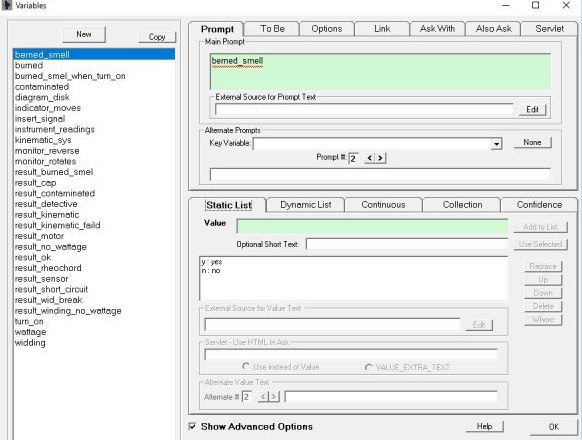
\includegraphics[scale = 1.35]{images/2.jpg}
	\caption{Список переменных заданной экспертной системы}
\end{figure}

\clearpage

\begin{figure}[h!]
	\centering
	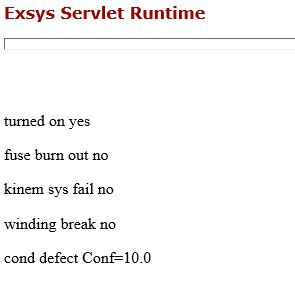
\includegraphics[scale = 0.7]{images/7_1.jpg}
	\caption{Пример работы системы}
\end{figure}




\section{Вывод}

В данной работе была изучена система для конструирования экспертных систем Exsys Corvid. Данная система имеет ряд достоинств:

\begin{itemize}
	\item Простота работы с системой.
	\item Наличие множества готовых шаблонных решений.
	\item Встроенные возможности для кастомизации.
\end{itemize}

А также набор недостатков:

\begin{itemize}
	\item Использование безнадежно устаревшей технологии Java Applet, что ставит крест на использование этой системы в реальных проектах.
	\item Платная лицензия, что вызывает недоумение ввиду предыдущего пункта.
	\item Ошибки в системе, которые обнаруживаются буквально при первом запуске.
	\item Не работает локализация (по крайней мере в 30-дневной версии).
	\item Сомнительная полезность. Система подходит только для простых шаблонных ЭС, в то время какв реальность может потребоваться интегрируемая ЭС в другой программный продукт или более кастомизированная версия.
\end{itemize}

К сожалению, недостатки Exsys Corvid в 2017 году значительно перевешивают преимущества. Весьма сомнительно, что кто-либо всерьез заинтересуется данной системой после ее использования, а уж тем более будет использовать ее в дальнейшем.

\section{Список литературы}

% \linebreak

\begin{flushleft}
	
[1] Exsys Corvid Expert System Demos [Электронный ресурс]. — URL: \href{http://www.exsys.com/demomain.html}{http://www.exsys.com/demomain.html} (дата обращения 09.11.2018). \linebreak

[2] ОБОЛОЧКА ЭКСПЕРТНЫХ СИСТЕМ EXSYS CORVID МЕТОДИЧЕСКОЕ ПОСОБИЕ [Электронный ресурс]. — URL: \href{http://faculty.ifmo.ru/csd/dimour/ES/Corvid.pdf}{http://faculty.ifmo.ru/csd/dimour/ES/Corvid.pdf} (дата обращения 09.11.2018). \linebreak

\end{flushleft}
	


\end{document}